\documentclass[11pt]{article}

% Change "review" to "final" to generate the final (sometimes called camera-ready) version.
% Change to "preprint" to generate a non-anonymous version with page numbers.
\usepackage[final]{acl}

% Standard package includes
\usepackage{times}
\usepackage{latexsym}
\usepackage[flushleft]{threeparttable} % http://ctan.org/pkg/threeparttable
\usepackage{booktabs,caption}

% For proper rendering and hyphenation of words containing Latin characters (including in bib files)
\usepackage[T1]{fontenc}
% For Vietnamese characters
% \usepackage[T5]{fontenc}
% See https://www.latex-project.org/help/documentation/encguide.pdf for other character sets

% This assumes your files are encoded as UTF8
\usepackage[utf8]{inputenc}

% This is not strictly necessary, and may be commented out,
% but it will improve the layout of the manuscript,
% and will typically save some space.
\usepackage{microtype}

% This is also not strictly necessary, and may be commented out.
% However, it will improve the aesthetics of text in
% the typewriter font.
\usepackage{inconsolata}

%Including images in your LaTeX document requires adding
%additional package(s)
\usepackage{graphicx}
\usepackage{svg}

% If the title and author information does not fit in the area allocated, uncomment the following
%
%\setlength\titlebox{<dim>}
%
% and set <dim> to something 5cm or larger.

\title{CAS 732: Replication Project Final Report}

% Author information can be set in various styles:
% For several authors from the same institution:
% \author{Author 1 \and ... \and Author n \\
%         Address line \\ ... \\ Address line}
% if the names do not fit well on one line use
%         Author 1 \\ {\bf Author 2} \\ ... \\ {\bf Author n} \\
% For authors from different institutions:
% \author{Author 1 \\ Address line \\  ... \\ Address line
%         \And  ... \And
%         Author n \\ Address line \\ ... \\ Address line}
% To start a separate ``row'' of authors use \AND, as in
% \author{Author 1 \\ Address line \\  ... \\ Address line
%         \AND
%         Author 2 \\ Address line \\ ... \\ Address line \And
%         Author 3 \\ Address line \\ ... \\ Address line}

\author{Samuel Khzym \\
  \texttt{khzyms@mcmaster.ca}}

%\author{
%  \textbf{First Author\textsuperscript{1}},
%  \textbf{Second Author\textsuperscript{1,2}},
%  \textbf{Third T. Author\textsuperscript{1}},
%  \textbf{Fourth Author\textsuperscript{1}},
% \\
%  \textbf{Fifth Author\textsuperscript{1,2}},
%  \textbf{Sixth Author\textsuperscript{1}},
%  \textbf{Seventh Author\textsuperscript{1}},
%  \textbf{Eighth Author \textsuperscript{1,2,3,4}},
% \\
%  \textbf{Ninth Author\textsuperscript{1}},
%  \textbf{Tenth Author\textsuperscript{1}},
%  \textbf{Eleventh E. Author\textsuperscript{1,2,3,4,5}},
%  \textbf{Twelfth Author\textsuperscript{1}},
% \\
%  \textbf{Thirteenth Author\textsuperscript{3}},
%  \textbf{Fourteenth F. Author\textsuperscript{2,4}},
%  \textbf{Fifteenth Author\textsuperscript{1}},
%  \textbf{Sixteenth Author\textsuperscript{1}},
% \\
%  \textbf{Seventeenth S. Author\textsuperscript{4,5}},
%  \textbf{Eighteenth Author\textsuperscript{3,4}},
%  \textbf{Nineteenth N. Author\textsuperscript{2,5}},
%  \textbf{Twentieth Author\textsuperscript{1}}
% \\
% \\
%  \textsuperscript{1}Affiliation 1,
%  \textsuperscript{2}Affiliation 2,
%  \textsuperscript{3}Affiliation 3,
%  \textsuperscript{4}Affiliation 4,
%  \textsuperscript{5}Affiliation 5
% \\
%  \small{
%    \textbf{Correspondence:} \href{mailto:email@domain}{email@domain}
%  }
% }

\begin{document}

\nolinenumbers

\maketitle

\section{Introduction}

The selected paper for replication is \textit{Transformer-XL: Attentive Language Models Beyond a Fixed-Length Context} \cite{dai2019transformerxlattentivelanguagemodels}, which augments the original transformer architecture with a recurrence mechanism. This allows it to overcome the limitation of losing information between segmented sections of the text, thus allowing for higher coherence over a longer context window. The code is publicly available at the following GitHub repo: \url{github.com/kimiyoung/transformer-xl}. My fork with the modifications and analysis done for this project can be found at \url{github.com/SamKhzym/transformer-xl}.

The paper uses open datasets with longer contexts to train (WikiText-103, enwik8, text8, One Billion Word, and Penn Treebank), and demonstrates lower perplexity (PPL) and bits-per-character (BPC) scores than other state-of-the-art methods of the time. It also shows better relative effective context length (RECL), which is a paper-defined metric, compared to other methods.

My replication experiments aim to verify two results presented in the paper. The first is to attain similar BPC and PPL values on two model sizes (41M, 150M) trained on two different datasets (\verb|enwik8|, \verb|wikitext-103|). 

\section{Related Work}

This paper is built off the original transformer architecture \cite{vaswani2023attentionneed}. This paper introduced the attention mechanism, which provides a more sophisticated and effective method for determining how relevant all other tokens in a segment of input tokens are to a specific token within that segment. This is very effective to allow for contextual understanding over a relatively short window, but the authors note that semantic information over longer context windows are generally lost since the attention mechanism does not consider any information before the current segment.

The paper compares their implementation of an extended context window with the "vanilla transformer", in which information is chunked into distinct segments and information cannot pass forward or backward between the segments, effectively eliminating any possibility of long context learning. One such paper that implemented this and obtained metrics on the same benchmarks measured by this paper did this with character-level language modeling \cite{alrfou2018characterlevellanguagemodelingdeeper}. This paper compares their implementation to several other SOTA methods of the time.

Another innovation the paper introduces to allow for significantly faster compute is to cache previously computed hidden states by using a relative positional encoding instead of an absolute one within a segment. This builds off a derivation of relative positional encodings from a previous paper on machine translation, also from the Google Brain team \cite{shaw2018selfattentionrelativepositionrepresentations}.

An alternate approach at the time to encoding global context within local segments includes using a topic compositional neural language model to determine the global semantic information of the entire document and include it in a Mixture-of-Experts architecture \cite{wang2018topiccompositionalneurallanguage}.

\section{Datasets}

The paper used the following public datasets which will be used for reproduction. The paper used additional datasets, but the replication project will only endeavour to use these two. These are great datasets for benchmarking performance compared to other language models, since many other papers use these same datasets for their own experiments.

\begin{itemize}
\item WikiText-103: Set of over 100M tokens extracted from Wikipedia articles.
\item enwik8: Raw character dump of English Wikipedia articles.
\end{itemize}

\subsection{enwiki8}

This dataset contains byte-level encodings of a raw dump of the first $10^8$ (95 MB) characters of English Wikipedia (delimiters, metadata, and everything). This dataset is commonly used for data compression experiments, with a general thought in the NLP space that the effectiveness of a language model is correlated with its ability to compress information. This is where the intuition behind the BPC metric comes from, but it is debatable as to whether compression is a good metric to evaluate model performance or not \cite{schmidt2024tokenizationcompression}. A snippet of the raw dataset is shown in Figure \ref{fig:enwik8sample}.

\begin{figure}[!htbp]
\centering
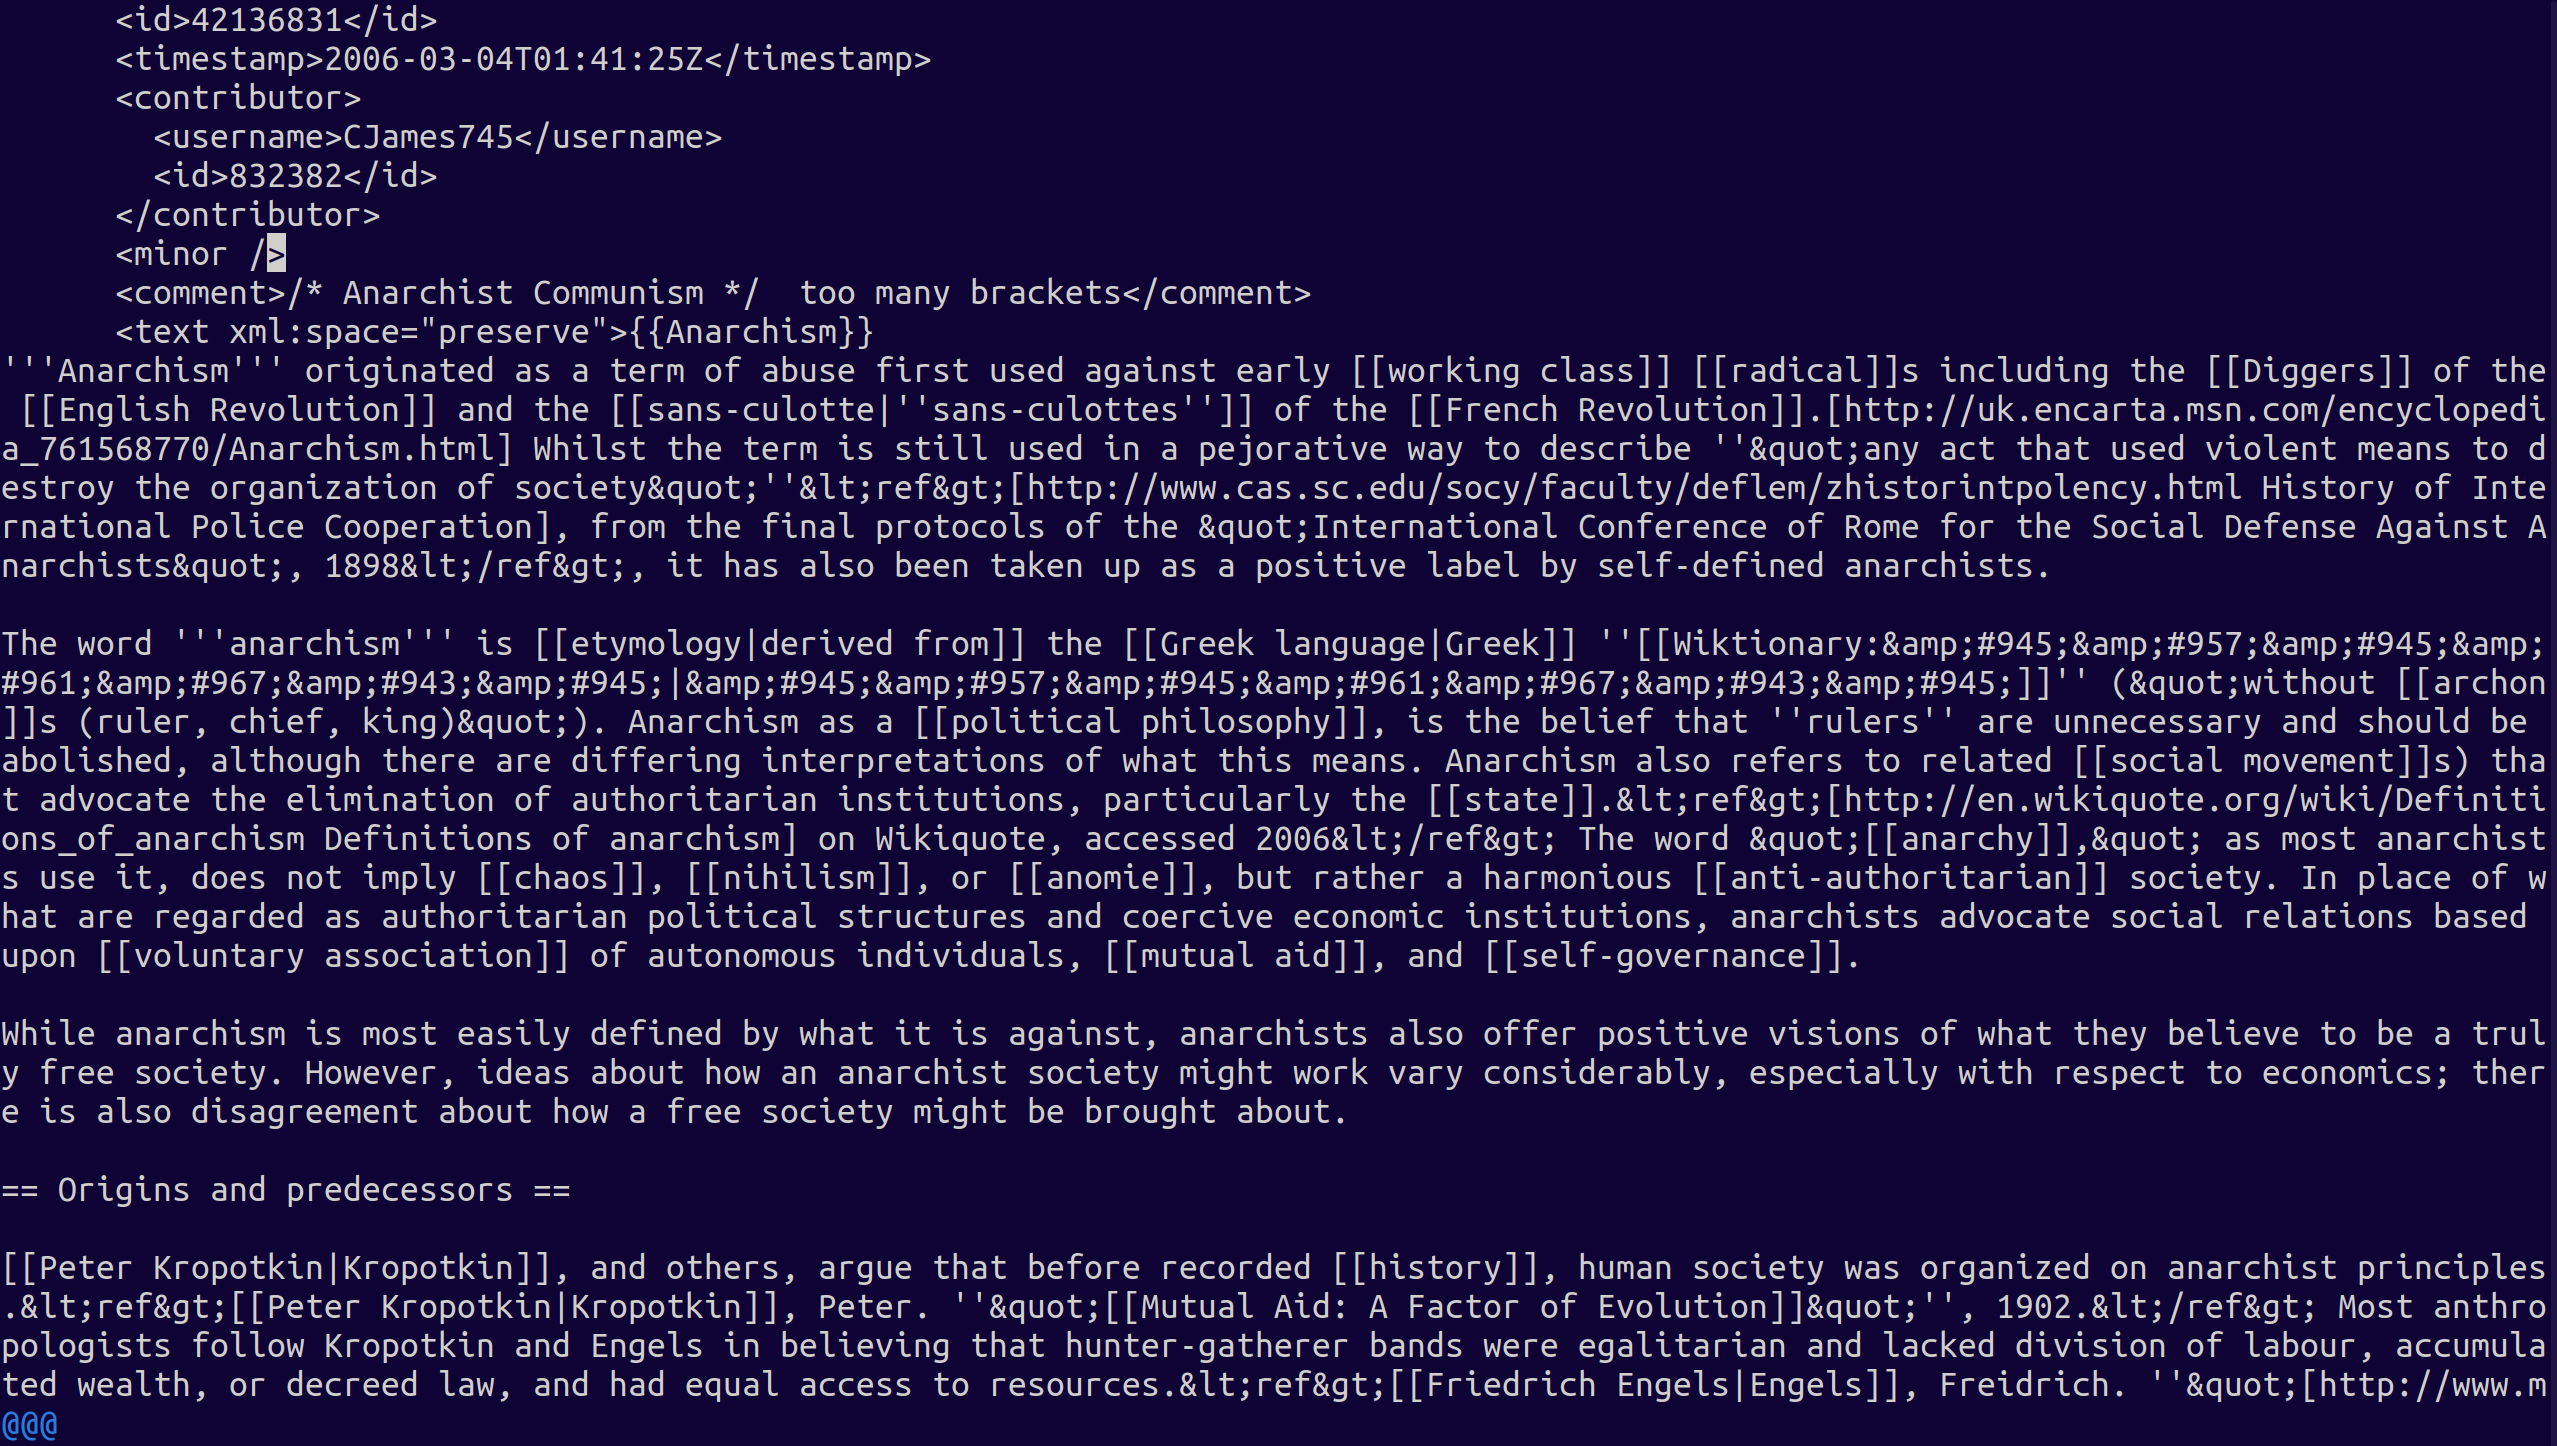
\includegraphics[width=0.45\textwidth]{img/enwik8_sample.png}
\caption{enwik8 Sample.}
\label{fig:enwik8sample}
\end{figure}

\subsection{WikiText-103}

This dataset contains 28,475 good and featured Wikipedia articles, with over 100 million English words. This dataset is commonly used for language modeling tasks that require long contexts, so it is a good application to the hypotheses the authors try to verify in this paper. It is more processed than enwik8, without most the delimeters and metadata of enwik8. The full uncompressed dataset is about 540 MB, so it is quite large. A snippet of the raw dataset is shown in Figure \ref{fig:wt103sample}.

\begin{figure}[!htbp]
\centering
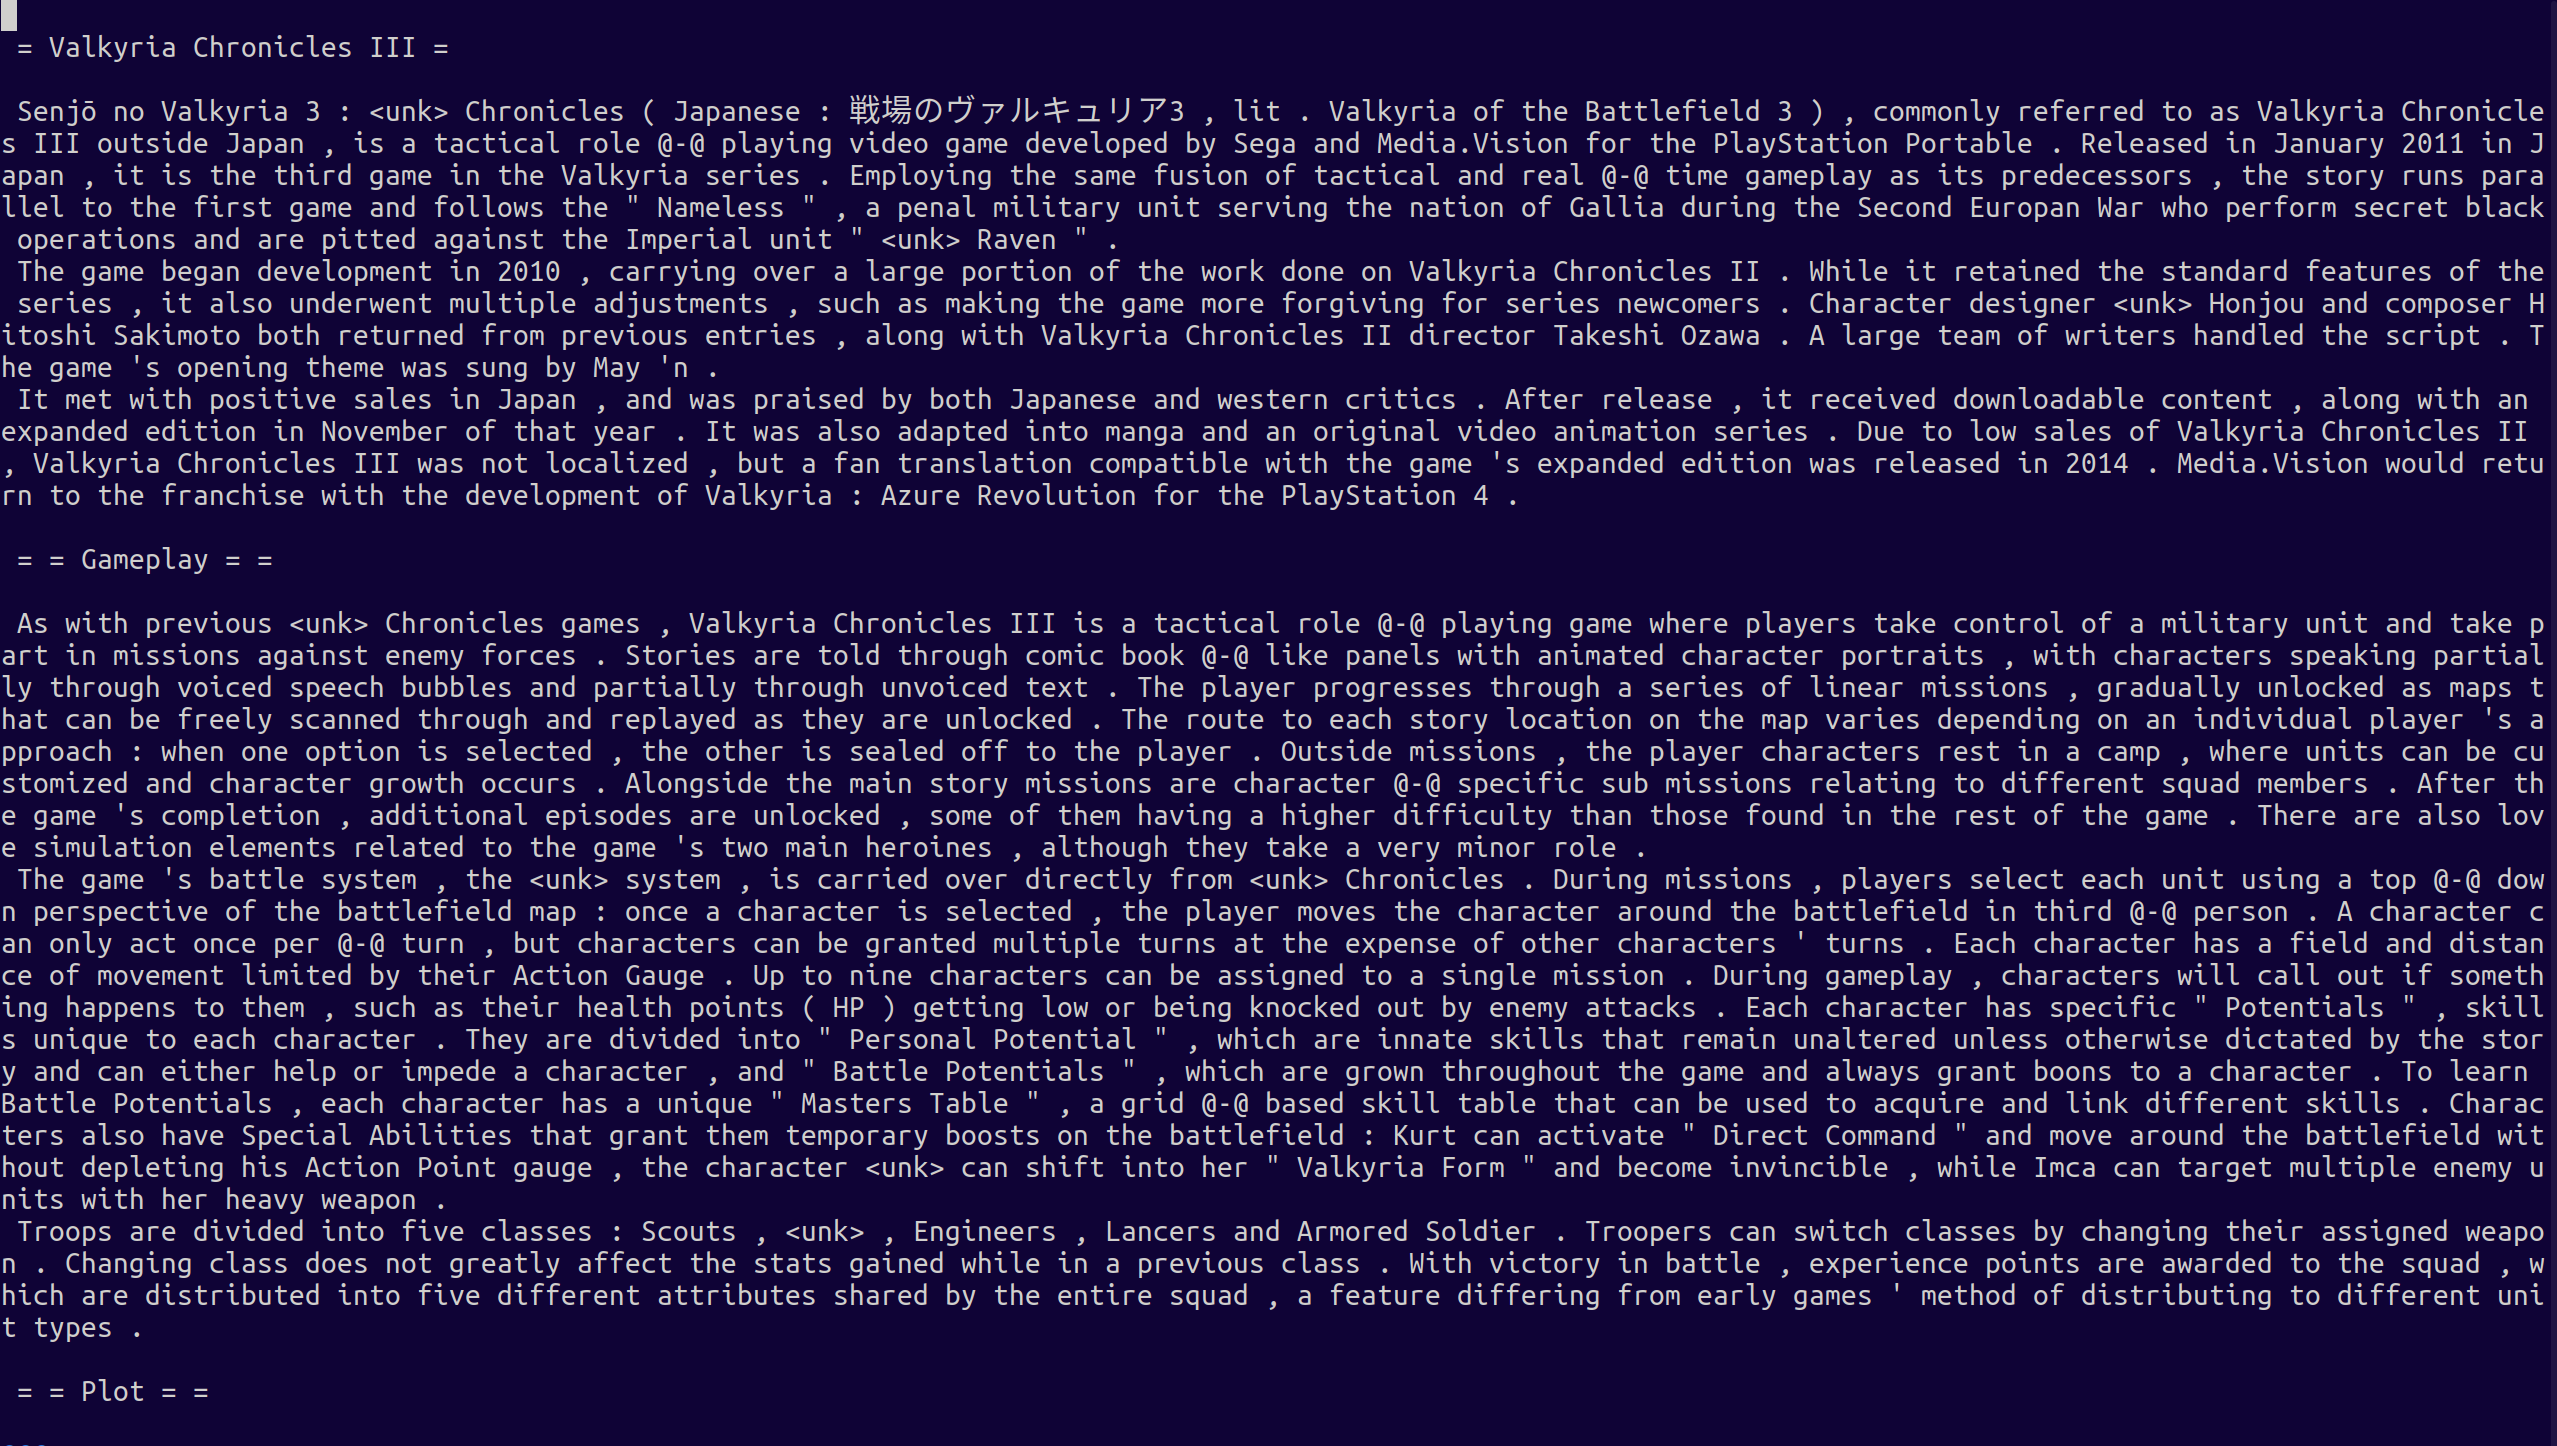
\includegraphics[width=0.45\textwidth]{img/wt-103_sample.png}
\caption{enwik8 Sample.}
\label{fig:wt103sample}
\end{figure}

\section{Datasets}

\subsection{Models}

The paper trained several sizes of models on different datasets, with the following names and number of parameters. Other sizes were trained, but the replication project will just attempt to train these ones.
\begin{itemize}
\item 12L Transformer-XL on enwik8 (41M). 
\item 16L Transformer-XL Standard on WikiText-103 (151M).
\end{itemize}

\subsection{Hypotheses}

The primary hypothesis the authors aim to verify is that this modified transformer architecture is superior to pre-existing methods on retaining long-context information. The verify this by achieving BPC and PPL metrics which were better than all comparison SOTA papers at the time. This does indicate that the model is better at predicting the next tokens in sequence, and therefore is a reasonable heuristic that longer context information is being retained.

They also experiment with the effect of different context lengths on the final perplexity scores and observe a sharp improvement as the context window starts increasing, and with diminishing returns past a context length of around 500, as shown in Figure \ref{fig:context_window} from the original paper.

\begin{figure}[!htbp]
\centering
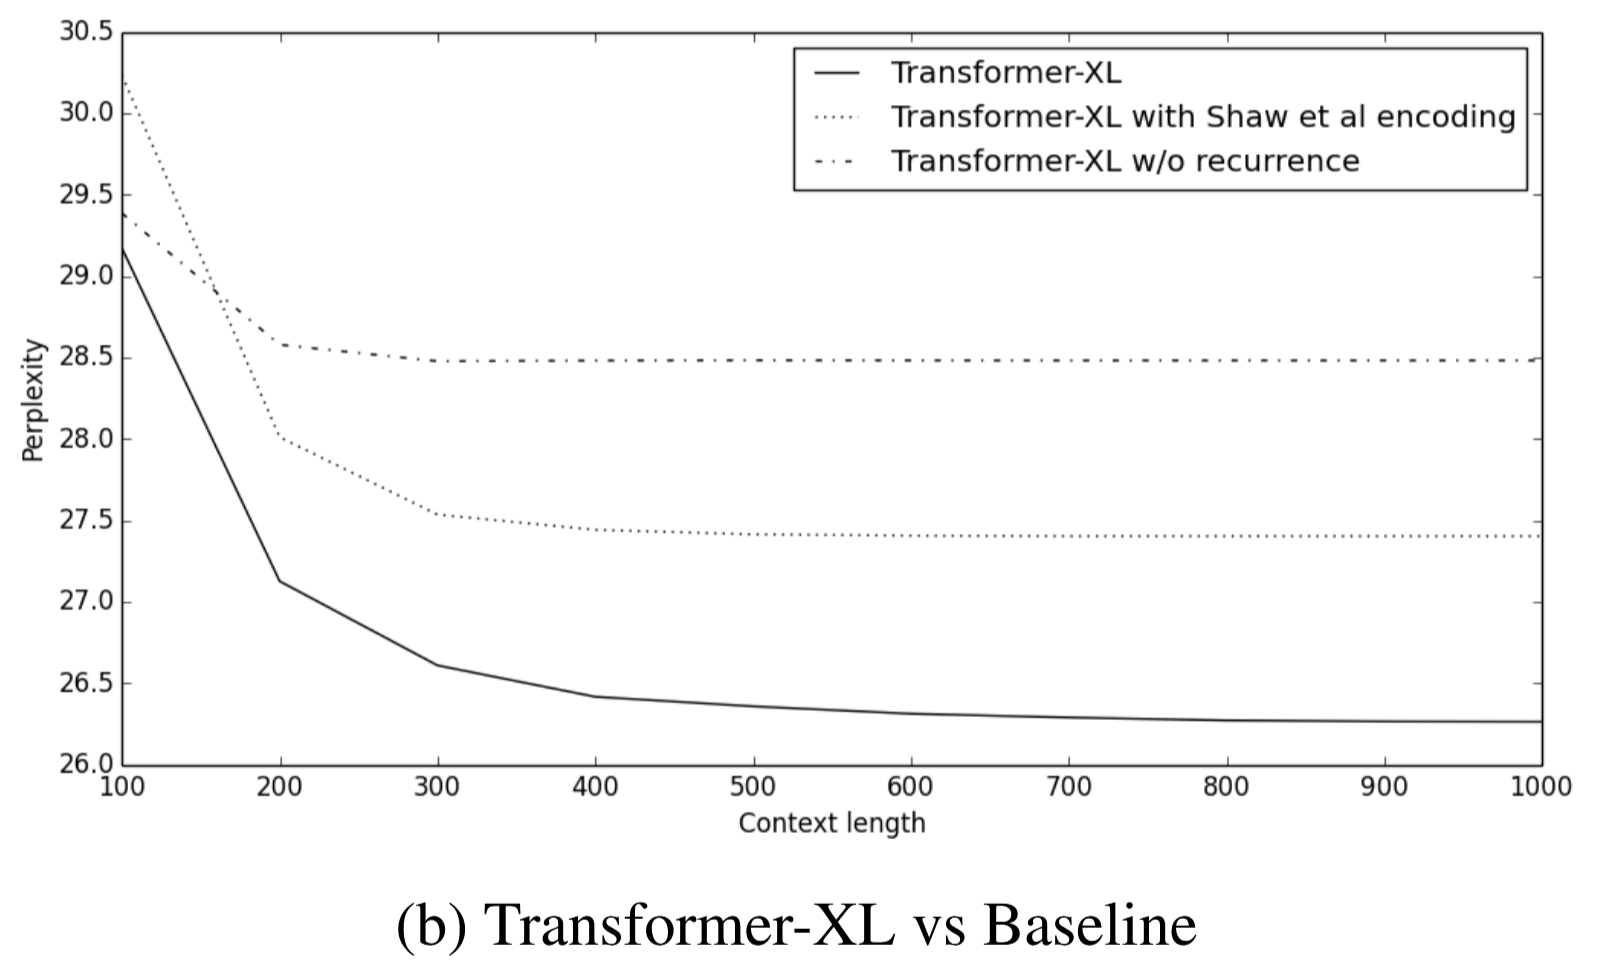
\includegraphics[width=0.5\textwidth]{img/context_length.png}
\caption{Perplexity Score vs. Training Context Legnth.}
\label{fig:context_window}
\end{figure}

\subsubsection{Hypothesis 1: Model Performance}

Results to replicate:

\begin{itemize}
\item Achieve a bits-per-character (bpc) score of $\sim 1.06$ ($\pm 10\%$) on the enwik8 dataset with the 41M parameter model (better than state-of-the-art of the time).
\item Achieve a perplexity score of $\sim 20.4$ ($\pm 10\%$) on the WikiText-103 dataset with the 151M parameter model (better than state-of-the-art of the time).
\end{itemize}

\subsubsection{Hypothesis 2: Context Window Diminishing Returns}

Re-train several versions of the model with varying context lengths to reproduce the graph in Figure \ref{fig:context_window}. More granularity may be applied in the context length breakpoints under evaluation for the sake of reducing training time.

\subsection{Authors' Implementation}

The authors implemented their novel model architecture using PyTorch with a distributed TPU cluster training setup. They also provided an alternate implementation in Python 2.7 with TensorFlow 1.12.0 which is setup to train on GPUs.

The authors provide several data management bash scripts to fetch all data from various servers, split them appropriately into train and test datasets, and cache them for efficient data loading.

Their software architecture is very modular in terms of how they structured the model. Most relevant model hyperparameters (number of layers, number of heads, segment size, context length, etc.) are arguments to the python script and are configurable in the provided bash scripts. The \verb|MEM_LEN| parameter controls the context window length.

\begin{figure}[!htbp]
\centering
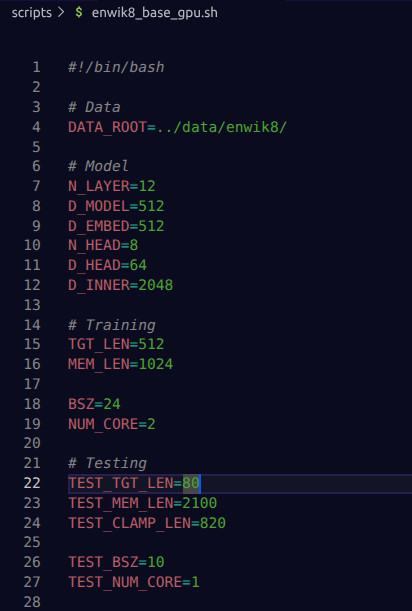
\includegraphics[width=0.33\textwidth]{img/training_options.png}
\caption{Training Script Options (Bash).}
\label{fig:training_options}
\end{figure}

\subsection{My Implementation}

I upgraded the codebase to TensorFlow 2.20.0 (most recent version) using TensorFlow's migration guide: \url{https://www.tensorflow.org/guide/migrate}. After working through several dependency issues, detailed in future sections, the training pipeline was working. I then cloned the repo on a McMaster department server \url{grace.cas.mcmaster.ca} with four NVIDIA H100 GPUs and used it to retrain the models from the ground up.

%% if time allows, add more details about tokenization and data loading, model architecture. maybe put in a diagram, might help to fill space.

Overall, it's a very serviceable codebase, but I found it challenging to trace the program flow. That's partially because I'm unfamiliar with TensorFlow, and also because the authors' implementation has several layers of abstraction to handle different training setups, and it was challenging to differentiate business logic from routing logic. That made modifications of the implementation particularly challenging.

\section{Results and Evaluation}

\subsection{Hypothesis 1: Model Performance}

\subsubsection{Pre-Trained Model Evaluation}

The paper provides shell scripts to fetch the pre-trained model checkpoints and data files from their website. The data and checkpoints are in the form of Python .pkl files, so the same Python versions as the authors are required to run the models and reproduce the results. Table \ref{tab:pretrained_results} shows the results of the pre-trained models compared to what is in the paper.

\begin{table}[!hbtp]
\begin{center}
\caption{Pre-Trained Model Checkpoints Results}
\label{tab:pretrained_results}
\begin{tabular}{ |c|c|c|c| }
 \hline
 Dataset & Metric & Paper & Repro. \\
 \hline
 WikiText-103 & PPL & 18.3 & 18.31 \\ 
 enwiki8 & BPC & 0.99 & 0.936* \\ 
 One Billion Word & PPL & 21.8 & 21.77 \\ 
 text8 & BPC & 1.08 & 1.15** \\
 \hline
\end{tabular}
\begin{tablenotes}
  \item[*] * Run on 300/4828 of total batches of dataset.
  \item[*] ** Run on 26/2442 of total batches of dataset.
  \end{tablenotes}
\end{center}
\end{table}

The paper's results match almost exactly with the model checkpoints provided by the authors. This is quite expected since I necessarily am running the same Python and TensorFlow version with the same models trained by the authors. The only discrepencies are the two datasets that were unable to run to completion (these ran for several hours). Since I am only able to run the original pre-trained models on CPU, that caused a major bottleneck in the inference time. 

The final values for both datasets that did not run to completion are relatively far from the final value, indicating to me there may be contiguous batches of the dataset where the model performs well (likely near the beginning since the reimplementation's result is significantly better than the paper's result), and some batches where it performs worse, likely later in the dataset.

\subsubsection{Retrained Model Evaluation}

\paragraph{12L Transformer-XL}

The 12L Transformer-XL model was trained on the enwik8 dataset for about 4.5 hours using all four GPUs. The final BPC value on the test dataset was 1.1476. A graph of BPC score over training steps is shown in Figure \ref{fig:enwik8_train}.

\begin{figure*}[!htbp]
\centering
\includesvg[width=\textwidth]{img/enwik8.svg}
\caption{Enwik8 BPC vs. Training Steps.}
\label{fig:enwik8_train}
\end{figure*}

This final BPC value is within 8.2\% of the reported value of the paper, thus meeting the 10\% error threshold for a successful replication. The reason for the discrepancy between my results and the authors is likely because they trained it for far longer (400,000 training steps compared to my $\sim$ 73,000), thus giving more time for the training curve to be driven further down. As shown in Figure \ref{fig:enwik8_train}, the training curve has an observable negative slope, and so it's reasonable to assume the model training has not fully plateaued at this point.

\paragraph{16L Transformer-XL Standard}

The 12L Transformer-XL model was trained on the enwik8 dataset for about 7.5 hours using all four GPUs. The final PPL value on the test dataset was 29.70. A graph of PPL score over training steps is shown in Figure \ref{fig:wt103_train}.

\begin{figure*}[!htbp]
\centering
\includesvg[width=\textwidth]{img/wt-103.svg}
\caption{WikiText-103 PPL vs. Training Steps.}
\label{fig:wt103_train}
\end{figure*}

This final PPL value is within 23.7\% of the reported value of the paper, missing the 10\% error threshold for a successful replication. The reason for the more major discrepancy between my results and the authors is likely because they trained it for far longer (400,000 training steps compared to my $\sim$ 55,000), thus giving more time for the training curve to be driven further down. As shown in Figure \ref{fig:wt103_train}, the training curve has an observable negative slope, and so it's reasonable to assume the model training has not fully plateaued at this point.

\subsection{Hypothesis 2: Context Window Diminishing Returns}

To test this hypothesis, five different 12L Transformer-XL models were trained on the enwik8 dataset for 10,000 training steps with varying context windows. The context windows tried were 0, 128, 256, 512, and 1024. The perplexity score vs. training step curve for all five models is shown in Figure \ref{fig:enwik8_context_length_experiments}. It is clear that a larger context window does cause the training perplexity to decrease faster, with clear diminishing returns especially between the 256 and 512 context lengths. 

Interestingly, the 512 to 1024 decrease in PPL score was better than expected in the original paper's results (Figure \ref{fig:context_window}), indicating that it had not fully plateaued. This may be because the models were only trained for 10,000 iterations instead of the 400,000 done in the original paper. Figure \ref{fig:ppl_vs_context_window} shows a reproduction of the graph in the original paper. The diminishing returns are clearly evident. The authors also may have used a different dataset/model to train the different variations. The enwik8 dataset was chosen for the purposes of the reproduction since it was the smallest dataset of the ones under test, and thus the quickest to train.

\begin{figure*}[!htbp]
\centering
\includesvg[width=\textwidth]{img/enwik8_contexts.svg}
\caption{PPL vs. Training Steps Over Different Context Windows.}
\label{fig:enwik8_context_length_experiments}
\end{figure*}

\begin{figure*}[!htbp]
\centering
\includesvg[width=\textwidth]{img/enwik8_contexts_repro.svg}
\caption{PPL vs. Context Window.}
\label{fig:ppl_vs_context_window}
\end{figure*}

\subsection{Evaluation of Reproducibility}

Overall, the results presented in the paper were relatively easy to reproduce, with both the pre-trained model checkpoints provided by the authors and the nicely setup data fetching and model training scripts. The code was clearly written to be reuseable and applied to other kinds of projects as well. 

An interesting additional insight I got in running the reproducibility experiments is seeing how quickly the different models converged with different context lengths. In Figure \ref{fig:enwik8_context_length_experiments}, the longer context models not only had a lower overall value than the model without context, but it also converged much faster from the start, showing the gains from the attention mechanism are immediately realizable in the training phase, while also driving the final value lower as the training process continues.

\section{Reflections}

\subsection{Technical Challenges}

The WikiText-103 dataset was not available from the download scripts due to the hosting site being taken down. I was able to find the same files at \hyperlink{https://www.kaggle.com/datasets/rohitgr/wikitext}{this Kaggle website}.

The major challenge with re-running the code provided by the authors is the old tech stack used being incompatible with my and the compute server's systems. I am running on Ubuntu 22.04, with an NVIDIA GTX 3070 GPU. The oldest version of CUDA that is supported for my operating system is CUDA 11.7, while the version required for TensorFlow 1.12.0 GPU is 9.0. I tried running the official docker image for TensorFlow 1.12.0 which has CUDA 9.0 pre-installed, but ran into CUDA mismatch related errors. 

The department server also does not support TensorFlow 1.12.0, and it does not have Docker installed. I tried running with Podman instead, but was not able to access the GPUs from the Podman infrastructure. The only options I had at that point were to try to find a combination of dependencies that worked on my system which supported the old tech stack (which was especially challenging given the many layers of compatability the softwares I was working with required), or to upgrade the code.

\subsubsection{Pre-Trained Model Checkpoints}

The only way I could run the model checkpoints and load from the .pkl files provided for baseline pre-trained model evaluation would be by running in CPU only, which is significantly slower and is the reason why the entire batch set could not be completed in Table \ref{tab:pretrained_results}. To do this, I ran the CPU only Tensorflow 1.12.0 docker image instead, which gave me no problems but ultimately resulted in me being unable to complete the entire batches.

\subsubsection{Model Retraining Pipeline (Local)}

Since running with a GPU is effectively required to retrain the models from scratch with any kind of efficiency, it was imperative to upgrade the tech stack used in the paper. To begin, migrating to a newer version of Python and TensorFlow was required to allow my system to utilize the GPU. However, the code was written before TensforFlow 2.0.0 was released, so I needed to follow the TensorFlow 1.0 to 2.0 migration guide (\verb|www.tensorflow.org/guide/migrate|). Once this was done, I needed to run a TensorFlow 2.15.0 Docker container, and I was able to run the updated code. However, due to out of memory issues, the model sizes provided natively were too large to run. 

For the text8 base model, for example, I had to halve the dimensions of the \verb|D_MODEL|, \verb|D_EMBED|, \verb|TGT_LEN|, and \verb|MEM_LEN| parameters, effectively reducing the model size by a considerable amount so it could fit in memory. This will result in a model that performs worse than the baseline would suggest. This version worked for running the training scripts, but the model was too large to fit in memory. Halving some model parameters resulted in a model that was able to fit in memory, but had half the parameters (40.9M to 20.5M). 

In theory, I calculated the number of weights and the size of the dataset, and I thought it should have been able to fit in memory, but I did not consider that the hidden states would constantly need to be cached in memory, thus dramatically increasing the required memory to get the training pipeline to work. Figure \ref{fig:TOO_MUCH_MEMORY} shows the memory usage once it was all working on the department server, it was way more than anticipated, over 200 GB of memory over the four GPUs. I had no hope to run this locally using the 8 GB of VRAM in my GPU and needed to turn to the department server.

\begin{figure}[!htbp]
\centering
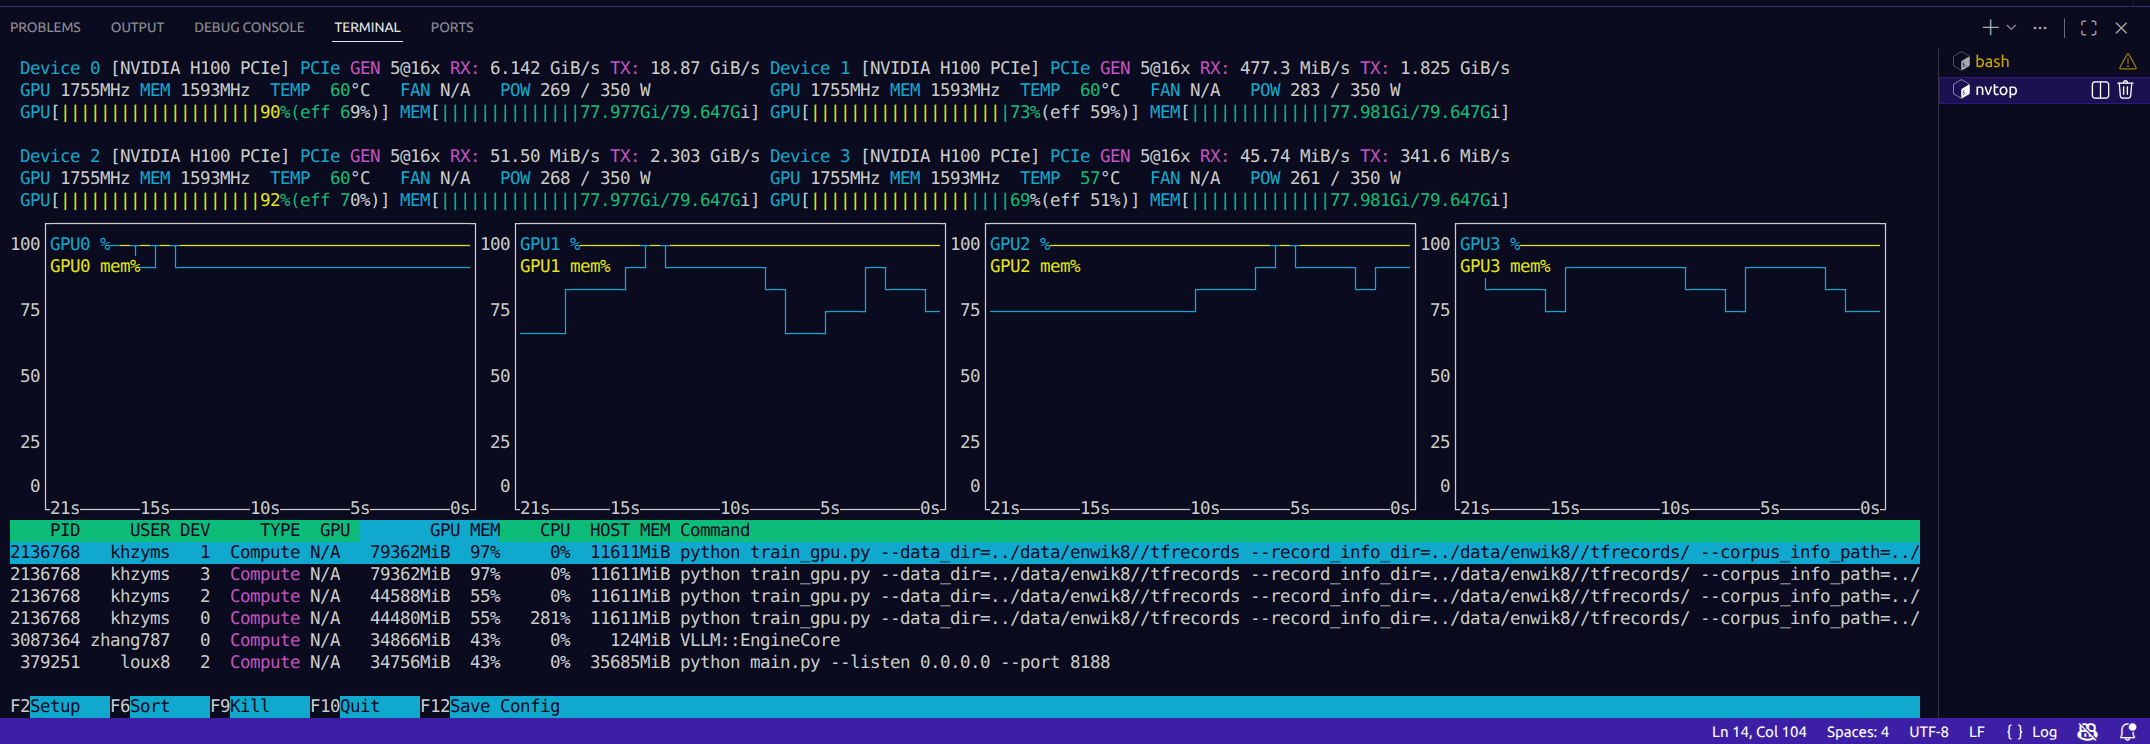
\includegraphics[width=0.45\textwidth]{img/too_much_memory.png}
\caption{Memory Usage on Department Server.}
\label{fig:TOO_MUCH_MEMORY}
\end{figure}

\subsubsection{Model Retraining Pipeline (Server)}

Since Docker was not available on the remote server and Podman was not allowing me to access the GPUs, I needed to create a Python virtual environment which comprised solely of compatible Python dependencies. This requires TensorFlow 2.20.0, which also required Keras 3.0, thus requiring minor refactoring of the original codebase since it did not originally use Keras. Once I worked through those issues, I needed to forcefully enable a few deprecated features to avoid the model crashing. Notably, the environment variable \verb|TF_USE_LEGACY_KERAS| needed to be set to 1 forcefully in the Python files, and Eager Execution needed to be manually disabled by using \verb|tf.compat.v1.disable_eager_execution()|. Once that all worked and a couple more minor bugs from the migration were resolved, the pipeline worked seamlessly.

\subsection{Additional Reflections}

Overall, I think this project was a very cool way to dive into more of the practical aspects of NLP research. I found it very interesting how this field centralizes a lot of the SOTA research and datasets through HuggingFace and ACL Anthology. It made referencing existing literature much more streamlined compared to other research fields I've worked on. Notably, autonomous driving research contains many proprietary datasets collected on research vehicles that cannot be uploaded, so the fact that the majority of the common datasets in the NLP community are so open was a pleasant surprise. I think it also contributes to fast pace of work accomplished in this field, with breakthroughs seemingly happening all the time in recent years.

I also discovered the trouble in trying to reproduce results from older models due to the lack of interoperability with model training pipelines. CUDA was notably the worst, being a very large library that is not backwards or forward compatible with many versions of Ubuntu or other libraries. In the past, I had tried running other peoples' machine learning models on my own machine (YOLO), but they were all up-to-date. Going through this made me realize how challenging migrating old codebases to newer frameworks was.

\section{Suggestions for Future Work}
I think the ideas in this paper are quite solid and a very simple addition to the transformer architecture to improve both runtime execution by caching previous hidden states, and overall performance, as shown by the gains in training runs. I would be curious to apply this mechanism to more modern architectures using the transformer if it is not already in use and see if there are any additional gains to those models as well. Having a PyTorch implementation that does not require TPUs would also be very nice since many modern implementations rely on PyTorch and use GPUs.

I also think it would be good to validate the results between different datasets instead of evaluating and training models on the same dataset, which it seemed the paper did quite frequently. The BPC metric in particular was interesting to me that it was so highly considered in this paaper, since it is more of a compression metric, and I'm not thoroughly convinced that better compression necessarily translates to better overall model performance, especially in dealing with data coming from outside the original distribution.

I would also like to see the code extended to be able to take in arbitrary queries examples from the user as opposed to just evaluating on the test dataset, and see the qualitative effectiveness of the next-word prediction task with various incomplete sentences that I can make up. This would help to put some intuition to how the metrics provided actually tie to qualitative model performance and usefulness.

\section{Disclosure of Generative AI Usage}

Google Gemini was used to help with the codebase migration to an upgraded version and explain some of the concepts in the original paper that I did not fully understand. All the analysis code and writing in this report is my own.

\bibliography{./references}

\end{document}
